% MATH 2551-L Final (Version A) --- fragment for \texttt{\textbackslash begin\{questions\}} in \texttt{exam-test/main.tex}.
% Course boilerplate lives on \texttt{\textbackslash exammodulecover}; this file is the problem set only.
\runningheader{Multivariable Calculus}{Practice Exam}{Page \thepage\ of \numpages}

\begingradingrange{calc03}

\newcommand{\tfblank}{\fillin[\mbox{\hspace{1.0em}}][2.2em]}
 
\question
Fill \textbf{T} in the blank if the statement is true; otherwise fill \textbf{F}.
\begin{parts}
  \part[4]
  \tfblank\ If $f(x,y)$ is defined on a closed and bounded region $R$ in the plane, then the extreme points of $f(x,y)$ only occur at critical points.

  \part[4]
  \tfblank\ Let $S{:}\ \vec{r}(x,y)=x\,\hat{\mathbf{\imath}}+y\,\hat{\mathbf{\jmath}}+f(x,y)\,\hat{\mathbf{k}}$ be a surface defined by $z=f(x,y)$. Then the surface area of $S$ is
  \[
    \iint_{R} \sqrt{f_x^{2}+f_y^{2}+1}\,dx\,dy
  \]
  where $R$ is the shadow in the $xy$-plane.

  \part[4]
  \tfblank\ Let $C$ be a curve with parametrization $\vec{r}(t)$ and let $\vec{T}(t)$ be the unit tangent vector at $t$. Then the curvature $\kappa$ (at $t$) is the length of $\dfrac{d\vec{T}}{ds}$, where $s$ is the arc length parameter with base point $\vec{r}(t_0)$ for some real number $t_0$.

  \part[4]
  \tfblank\ Let $D$ be a (closed) ball of radius $a$. The volume of $D$ is
  \[
    \int_{0}^{2\pi}\int_{0}^{a}\int_{-\sqrt{a^{2}-r^{2}}}^{\sqrt{a^{2}-r^{2}}} r\,dz\,dr\,d\theta .
  \]

  \part[4]
  \tfblank\ Let $\vec{u}$, $\vec{v}$, and $\vec{w}$ be nonzero vectors. If $\vec{u}\times\vec{v}=\vec{u}\times\vec{w}$,   then $\vec{v}=\vec{w}$.
\end{parts}


\question
Compute the following and write your results on the answer lines. Show all work.
\begin{parts}
  \part[4]
  Evaluate
  \[
    \int_{0}^{1}\Bigl(6t e^{2t^{2}}\Bigr)\hat{\mathbf{\imath}}+\bigl(\ln(t+1)\bigr)\hat{\mathbf{\jmath}}+(\sin\pi t)\,\hat{\mathbf{k}}\,dt .
  \]

  \smallskip
  \makeemptybox{1.25in}

  \part[4]
  Find
  \[
    \frac{d}{dt}\Bigl((\ln t)\,\hat{\mathbf{\imath}}+\bigl(e^{\cos t}\bigr)\hat{\mathbf{\jmath}}+(\sin 2t)\,\hat{\mathbf{k}}\Bigr).
  \]

  \smallskip
  \makeemptybox{1.25in}

  \part[4]
  Evaluate $\displaystyle\int_{0}^{6}\int_{y^{2}/6}^{4y} dx\,dy$.

  \smallskip
  \makeemptybox{1.25in}

  \part[4]
  Let $2z^{3}-xy+3yz+y^{3}-52=0$. Find $\dfrac{\partial z}{\partial x}$ at $(3,3,2)$.

  \smallskip
  \makeemptybox{1.25in}

  \part[4]
  Evaluate $\displaystyle\int_{C}(x+y+z)\,ds$ where $C$ is the straight line segment from $(4,2,3)$ to $(3,-1,-1)$.

  \smallskip
  \makeemptybox{1.25in}

  \part[4]
  Compute $(2\hat{\mathbf{\imath}}+\hat{\mathbf{\jmath}}+3\hat{\mathbf{k}})\times(\hat{\mathbf{\imath}}+2\hat{\mathbf{\jmath}}+\hat{\mathbf{k}})$.

  \smallskip
  \makeemptybox{1.25in}
\end{parts}

\newpage

\question
Let $\displaystyle\vec{F}=\frac{1}{y}\,\hat{\mathbf{\imath}}+\Bigl(\frac{1}{z}-\frac{x}{y^{2}}\Bigr)\hat{\mathbf{\jmath}}-\frac{y}{z^{2}}\,\hat{\mathbf{k}}$ be a vector field in space.
\begin{parts}
  \part[6]
  Show that $\vec{F}$ is conservative using the component test.

  \smallskip
  \makeemptybox{2in}

  \part[6]
  Find a potential function $f(x,y,z)$ for $\vec{F}$.

  \smallskip
  \makeemptybox{2in}

  \part[6]
  Suppose $\vec{F}$ is the velocity field of a fluid. Let
  \[
    \vec{r}(t)=\frac{1+t+2t^{2}}{2}\,\hat{\mathbf{\imath}}+(1+t)\,\hat{\mathbf{\jmath}}+(1+t^{3})\,\hat{\mathbf{k}},\qquad 0\le t\le 1,
  \]
  be a path in space. Compute the flow of $\vec{F}$ along $\vec{r}(t)$.

  \smallskip
  \makeemptybox{2in}
\end{parts}

\newpage

\question
A quadric surface $S$ is given by $z^{2}=x^{2}+y^{2}$.
\begin{parts}
  \part[4]
  Determine the type of the quadric surface $S$.

  \smallskip
  \makeemptybox{1.25in}

  \part[5]
  Find a parametrization of the normal line $\ell$ at the point $P(1,0,-1)$.

  \smallskip
  \makeemptybox{1.5in}

  \part[5]
  Find the distance from the point $Q(2,3,5)$ to the normal line $\ell$ in part~(b).

  \smallskip
  \makeemptybox{1.5in}
\end{parts}

\newpage

\question
Let $g(x,y,z)=x^{2}+2y-z^{2}$ and $h(x,y)=2x e^{3y}$.
\begin{parts}
  \part[7]
  Find the minimum of $g(x,y,z)$ subject to $6x-y=0$ and $y+z=0$.

  \smallskip
  \makeemptybox{2.25in}

  \part[5]
  Find the quadratic (second-order) approximation of $h(x,y)$ near the origin.

  \smallskip
  \makeemptybox{1.5in}
\end{parts}

\newpage

\question
Let $C$ be the arc parametrized by
\[
  \vec{r}(t)=(\cos t+t\sin t)\,\hat{\mathbf{\imath}}+(\sin t-t\cos t)\,\hat{\mathbf{\jmath}}+3\,\hat{\mathbf{k}},\qquad 1\le t\le\pi .
\]
\begin{parts}
  \part[5]
  Find the unit tangent vector $\vec{T}(t)$ to $\vec{r}(t)$ at (arbitrary) $t$.

  \smallskip
  \makeemptybox{2in}

  \part[5]
  Find the torsion $\tau(t)$ of the curve at (arbitrary) $t$.

  \smallskip
  \makeemptybox{2in}

  \part[5]
  Compute the length of the arc $C$.

  \smallskip
  \makeemptybox{1.5in}
\end{parts}

\newpage

\question
Suppose $\vec{F}=(2xz)\,\hat{\mathbf{\imath}}+\bigl(1-4xy^{2}\bigr)\hat{\mathbf{\jmath}}+(2z-z^{2})\,\hat{\mathbf{k}}$. Let $D$ be the region bounded above by the elliptic paraboloid $z=6-2x^{2}-2y^{2}$ and below by the plane $z=0$. Let $S$ be the boundary surface of $D$, i.e.
\[
  S=\bigl\{(x,y,z): z=6-2x^{2}-2y^{2},\ 0\le z\le 6\bigr\}\ \cup\ \bigl\{(x,y,z): x^{2}+y^{2}\le 3,\ z=0\bigr\}.
\]
Let $C$ be the curve in the $xy$-plane defined by $x^{2}+y^{2}=3$.
\begin{parts}
  \part[9]
  Find the area of $S$. You may use the parametrizations
  \[
    \vec{r}_{\text{side}}(r,\theta)=\bigl(r\cos\theta,\,r\sin\theta,\,6-2r^{2}\bigr),\quad 0\le r\le\sqrt{3},\ 0\le\theta\le 2\pi
  \]
  for the side shell and
  \[
    \vec{r}_{\text{bottom}}(r,\theta)=\bigl(r\cos\theta,\,r\sin\theta,\,0\bigr),\quad 0\le r\le\sqrt{3},\ 0\le\theta\le 2\pi
  \]
  for the bottom of $S$.

  \smallskip
  \makeemptybox{1.5in}

  \part[7]
  Use the divergence theorem to find the outward flux of $\vec{F}$ across the boundary of $D$.

  \smallskip
  \makeemptybox{1.5in}

  \part[7]
  Use Green's theorem to find the counterclockwise circulation of $\vec{F}$ around $C$.

  \smallskip
  \makeemptybox{1.5in}
\end{parts}

\newpage

\question
Let $\displaystyle f(x,y)=\frac{x}{\sqrt{x^{2}+y^{2}}}$.
\begin{parts}
  \part[5]
  Find the domain of $f$. Is it open? Is it closed? Justify your answers.

  \smallskip
  \makeemptybox{2in}

  \part[6]
  Exhibit two paths to $(0,0)$ along which $f(x,y)$ has different limiting values, and conclude that $\lim_{(x,y)\to(0,0)} f(x,y)$ does not exist.

  \smallskip
  \makeemptybox{2.25in}
\end{parts}

\newpage

\question
Let $D$ be the solid bounded by $z=11-11(x^{2}+y^{2})$ and $z=(x^{2}+y^{2})^{2}-1$. Let $\delta(x,y,z)=6$ be the density of the solid.
\begin{parts}
  \part[7]
  Compute the volume of $D$ using cylindrical coordinates.

  \smallskip
  \makeemptybox{2.25in}

  \part[6]
  Compute the moment of inertia of the solid about the $z$-axis.

  \smallskip
  \makeemptybox{2.25in}
\end{parts}

\newpage

\bonusquestion
Let $C$ be the circle of radius $1$ with center $(3,0)$ in the $xz$-plane. Let $S$ be the surface obtained by rotating $C$ about the $z$-axis (a torus of revolution).
\begin{parts}
  \bonuspart[10]
  Find a parametrization of $S$.

  \smallskip
  \makeemptybox{2.5in}

  \bonuspart[5]
  Find the surface area of $S$.

  \smallskip
  \makeemptybox{2in}
\end{parts}

\begin{center}
  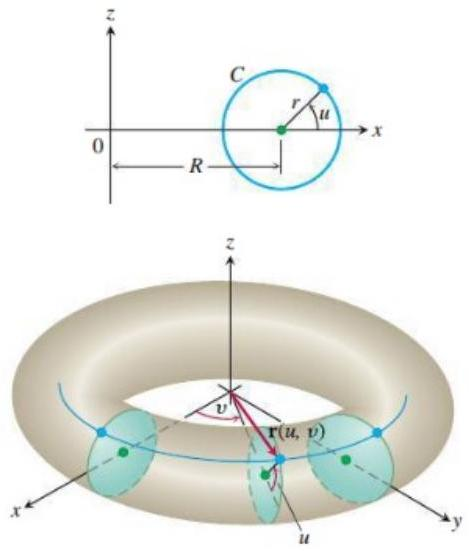
\includegraphics[width=0.40\linewidth]{images/bfcf5552-fe66-4f57-93c5-529d70a480ce-12_551_469_560_833}\\[0.35em]
  {\small\textit{Figure: torus of revolution}}
\end{center}

\endgradingrange{calc03}
